\documentclass[oneside]{VUMIFPSkursinis}
\usepackage{algorithmicx}
\usepackage{algorithm}
\usepackage{algpseudocode}
\usepackage{amsfonts}
\usepackage{float}
\usepackage{amsmath}
\usepackage{bm}
\usepackage{caption}
\usepackage{hyperref}
\usepackage{color}
\usepackage{float}
\usepackage{graphicx}
\usepackage{listings}
\usepackage{subfig}
\usepackage{ltablex}
\usepackage{longtable}
\usepackage{wrapfig}
\usepackage{enumitem}
\usepackage{subfig}
\usepackage{caption}
\usepackage{pbox}
\renewcommand{\labelenumii}{\theenumii}
\renewcommand{\theenumii}{\theenumi.\arabic{enumii}.}
\renewcommand{\labelenumiii}{\theenumiii}
\renewcommand{\theenumiii}{\theenumii\arabic{enumiii}.}
% Titulinio aprašas
\university{Vilniaus universitetas}
\faculty{Matematikos ir informatikos fakultetas}
\department{Programų sistemų katedra}
\papertype{Projektinis darbas}
\title{Internetinio banko tinklalapis}
\titleineng{Bankininkystė}
\status{3 kurso 3 grupės studentai}
\author{Justas Tvarijonas}
\secondauthor{Džiugas Mažulis}   
\thirdauthor{Michal Stankevič}   
\supervisor{Kristina Lapin, Doc., Dr.}
\date{Vilnius – \the\year}

\begin{document}
\maketitle
\sectionnonum{Anotacija}
\subsectionnonum{Darbo tikslas}
Įvertinti 3-ių sukurtų maketų panaudojamumą ir pateikti išvadas, kaip toliau tęsti projektą. Šiam tikslui įgyvendinti išsikėlėme šiuos uždavinius:
\begin{enumerate}
	\item Kiekvienam maketui atlikti euristinį tikrinimą,
	\item Kiekvienam maketui atlikti pažintinę peržvalgą,
	\item Nustatyti tolimesnę projekto eigos kryptį.
\end{enumerate}
\subsectionnonum{Darbo pasiskirstymas}
\begin{itemize}
	\item Justas Tvarijonas - tvarijonasjustas@gmail.com
	\item Džiugas Mažulis - džiugas.mažulis@gmail.com
	\item Michal Stankevič - michal.stankevic@gmail.com 
\end{itemize}
\tableofcontents
\sectionnonum{Įvadas}
\subsectionnonum{Dalykinė sritis}
Internetinė bankininkystė.
\subsectionnonum{Probleminė sritis}
Vartotojo grafinės sąsajos išmokstamumo gerinimas, pagrindinėms funkcijoms pasiekti atliekamų žingsnių bei klaidų mažinimas.
\subsectionnonum{Naudotojai}
Banko klientas - turi galimybę atlikti mokėjimus, peržiūrėti sąskaitos išrašus, kurti mokėjimo ruošinius, ieškoti reikalingos informacijos.
\subsectionnonum{Darbo pagrindas}
Trečiojo laboratorinio darbo reikalavimai.
\section{Džiugo Mažulio maketo vertinimas}
\subsection{Euristinis tikrinimas}
\begin{center}
	\begin{table}[h]
\begin{tabular}{|p{3.5cm}|p{3.5cm}|p{8.1cm}|}
  \hline
	Euristika & Defekto sunkumas & Komentaras \\ \hline
	Būsenos matomumas & Vidutinis & Vartotojas savo buvimo vietą mato tik būdamas pirmame hierarchijos sluoksnyje, jam einant į gylesnius sluoksnius, jis gali užmiršti kokioje vietoje yra. \\ \hline
	Sistemos atitikimas realiam pasauliui & Lengvas & Vietinių mokėjimų lange vartotojui gali būti ne akivaizdu, ką reiškia terminas "Gavėjo pavadinimas" \\ \hline
	Naudotojo valdomas dialogas & Vidutinis & Languose nėra grįžimo atgal mygtukų, vienintelis būdas grįžti yra naudojantis mygtukų juosta. \\ \hline
	Klaidų prevencija \label{lentele:klaiduPrevencijaJ} &\hyperref[fig:klaiduPrevencijaMygtukai]{Didelis} & Vietinių mokėjimų lange mygtukai "Patvirtinti mokėjimą" ir "Išsaugoti duomenis" nėra atskirti tarpais, bei paspaudus "Patvirtinti mokėjimą" nėra atliekamas papildomas paklausimas ar vartotojas nori atlikti tą mokėjimą, todėl yra galimybė, kad vartotojas norėdamas išsaugoti duomenis prieš savo valią atliks mokėjimo pavedimą\\ \hline
	& & \\ \hline
\end{tabular}
\caption{Justo Tvarijono vertinimas}
\end{table}
\end{center}

\begin{figure}[!htb]
	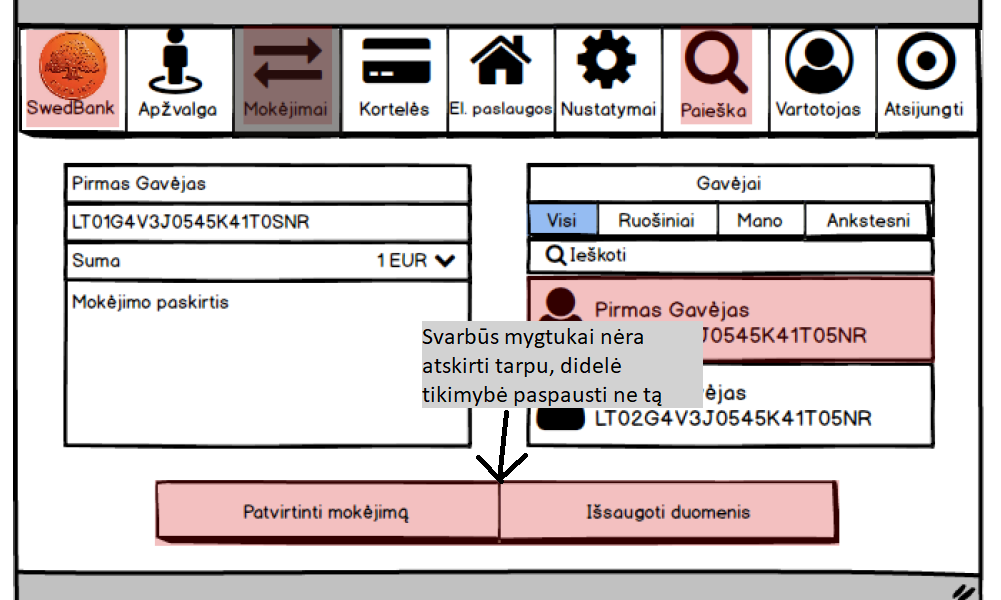
\includegraphics[scale=0.55]{MokejimoPatvirtinimasKlaiduPrevencija.png}
  \caption{Mygtukų išdėstymas vietinių mokėjimų lange}
	\label{fig:klaiduPrevencijaMygtukai}
\end{figure}
\hyperref[lentele:klaiduPrevencijaJ]{Defektas} yra didelės reikšmės, kadangi mokėjimo pavedimas yra rimta operacija, todėl klaidingas jos įvygdymas sukeltų reikšmingų nepatogumų sistemos naudotojui. Šią problemą galima spręsti keliais būdais: 1) mygtukus reiktų atitraukti į priešingas puses, kad tarp jų būtų tarpas užtikrinantis didesnį paspaudimų tikslumą. 2) prieš patvirtinant mokėjimą galima parodyti papildomą langą, kuriame vartotojas galėtų patvirtinti, kad nori atlikti šią operaciją.

\subsection{Pažintinė peržvalga}
\begin{center}
\begin{table}[h]
\begin{tabular}{|p{5cm}|p{5cm}|p{5cm}|}
	\hline
	Užduoties žingsniai & Ar aiškiai matoma, ką daryti? & Ar suprantamas atsakas? \\ \hline
\end{tabular}
\caption{Justo Tvarijono vertinimas}
\end{table}
\end{center}
\subsection{Apibendrinimas}
\section{Justo Tvarijono maketo vertinimas}
\subsection{Euristinis tikrinimas}
\subsection{Pažintinė peržvalga}
\subsection{Apibendrinimas}
\section{Michal Stankevič maketo vertinimas}
\subsection{Euristinis tikrinimas}
\subsection{Pažintinė peržvalga}
\subsection{Apibendrinimas}
\section{Išvados}
\end{document}
